\documentclass{article}
\usepackage[utf8]{inputenc}

\title{Discrete Systems}
\author{Carli Peters and Lindsay Amendola}
\date{22 December 2020}
\usepackage{indentfirst}
\usepackage{graphicx}
\begin{document}

\maketitle

\section{Introduction}
The topic that we did our final project on is discrete systems, which is basically a system with a number of states that somebody is able to count. Within discrete systems, changes occur in discrete steps. We can call these steps $k = 0,1,2,...i.$ The state of the system at time $i+1$ depends on the state of the system at all the previous times:
$$
n_{i+1}=f(n_0,n_1,n_2,...,n_i).
$$
These states can occur in multiple steps, as shown above, or can be done in a single step process:
$$
n_{i+1}=f(n_i)
$$
The single steps of the states in the system is also known as fixed point iteration and fixed point iteration is what is often used in the real world.
\subsection{Motivation}
A real life example on how discrete systems is used is seen in the medical field. In the modern world, people rely on medications to improve their health or heal a wound. When medication is prescribed to be taken daily, a new dosage enters the body everyday. However, each time a new dosage is taken, there is still some medication left in the body and it adds up in steps each time a dosage is taken until there is enough of the dosage in the body that the medicine no longer has to be taken. The medical professionals who are giving the patients the doses can use fixed point iteration to see how much of the dose is left from the previous day for each day going forward. These iterations can then be plotted on a cobweb plot, which shows us what is happening at each iteration, or in this case, each day the patient is receiving medicine. 
\begin{figure}
    \centering
    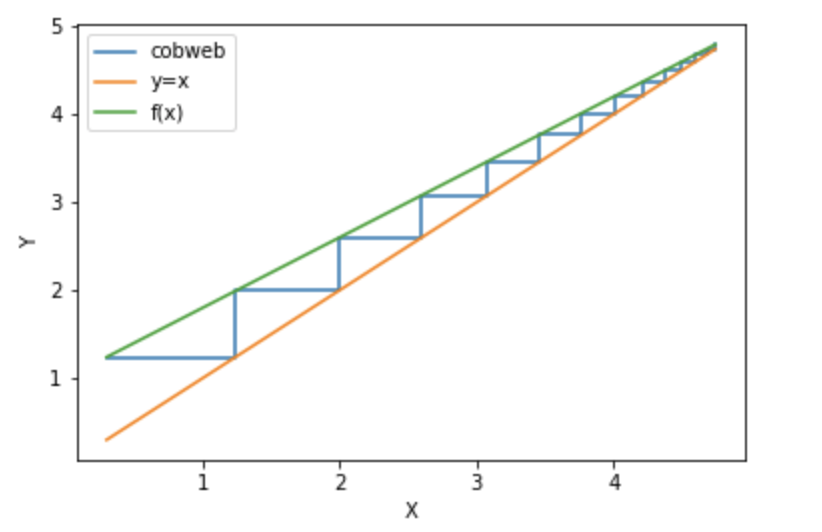
\includegraphics[width=8cm]{cobweb.png}
    \caption{This cobweb plot portrays how the fixed point iterations vary from day to day by taking discrete steps}
    \label{fig:Cobweb Plot for Medication Use}
\end{figure}

\subsection{Main Goals}
The main goals for the project are to see how each of the topics within discrete systems relate to one another. From the first instance that was shown, which was how changes occur in discrete steps, we can then use that to look into other important points with discrete systems. Using the equation $n_{i+1}=f(n_0,n_1,n_2,...,n_i)$, we can see the iterations within cobweb plots, which then leads into other forms of convergence as well. Discrete systems can also converge into patterns, which is seen in period 3 cycles that converge to three points and repeats every three iterations and then with bifurcation, which contains multiple fixed points.

\subsection{Brief Summary}
Throughout the rest of the paper, we will be talking about the approaches we took to obtain the result of seeing how all the points in discrete systems relate to one another. We will go more in depth about cobweb plots, which show the reader what is happening at each iteration. This then leads into period 3 cycles, which is a system that converges to a sequence of three points rather than one fixed point. An image of this instance is shown in Figure 2:
\begin{figure}[htp]
    \centering
    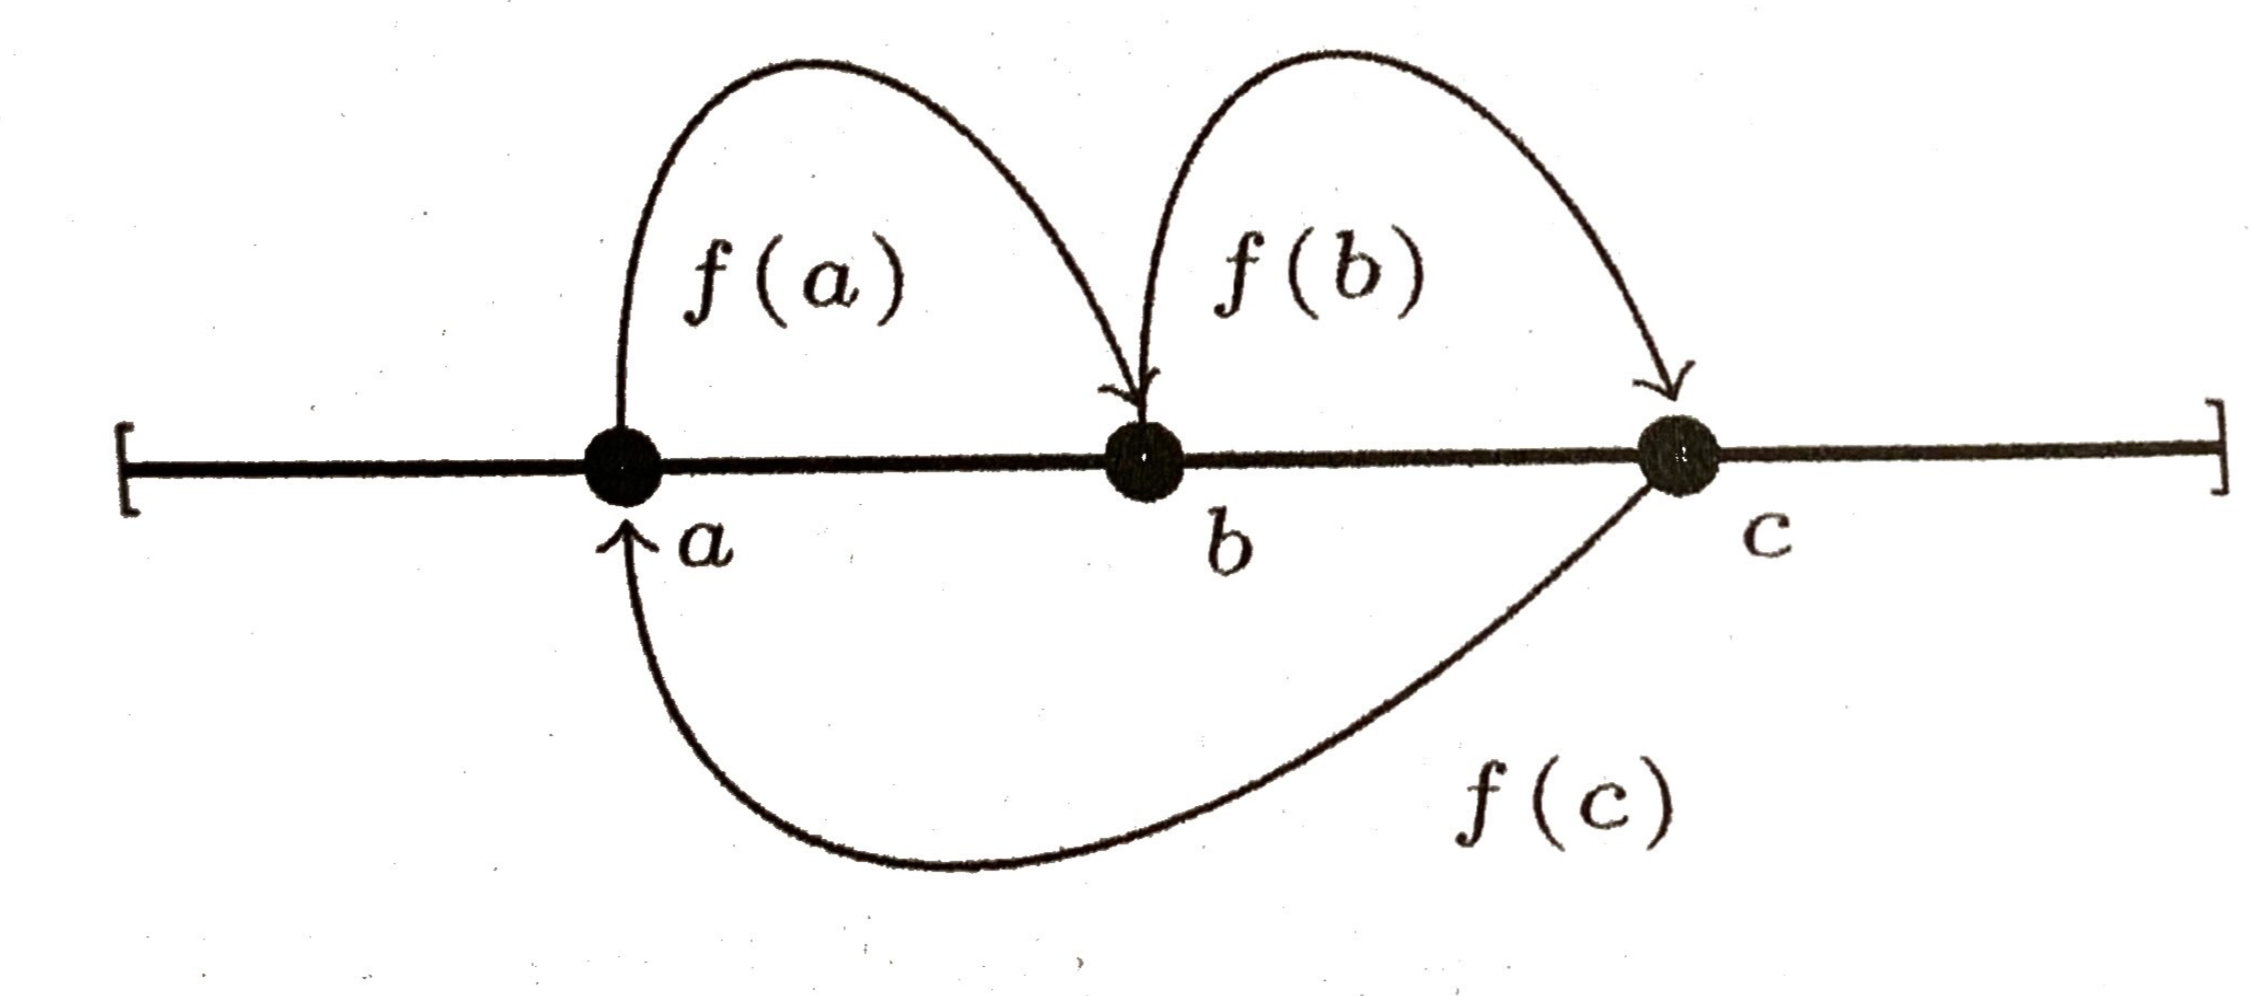
\includegraphics[width=8cm]{period3cycle.png}
    \caption{This portrays the system converging to a sequence of 3 points}
    \label{fig:Period 3 Cycle}
\end{figure}

Sometimes, discrete systems do not converge to one fixed point or go in a cycle of converging to the same three points. This is then indicating chaos, which is then looked into using a logistic map, which uses the equation:
$$
x_{n+1}=ax_n(1-x_n)
$$
Logistic maps can also help us see when bifurcation takes place, which is when two or more points tend to suddenly appear when $a$ is increased past 3. An image of a bifurcation diagram is shown in figure 3:
\begin{figure}[htp]
    \centering
    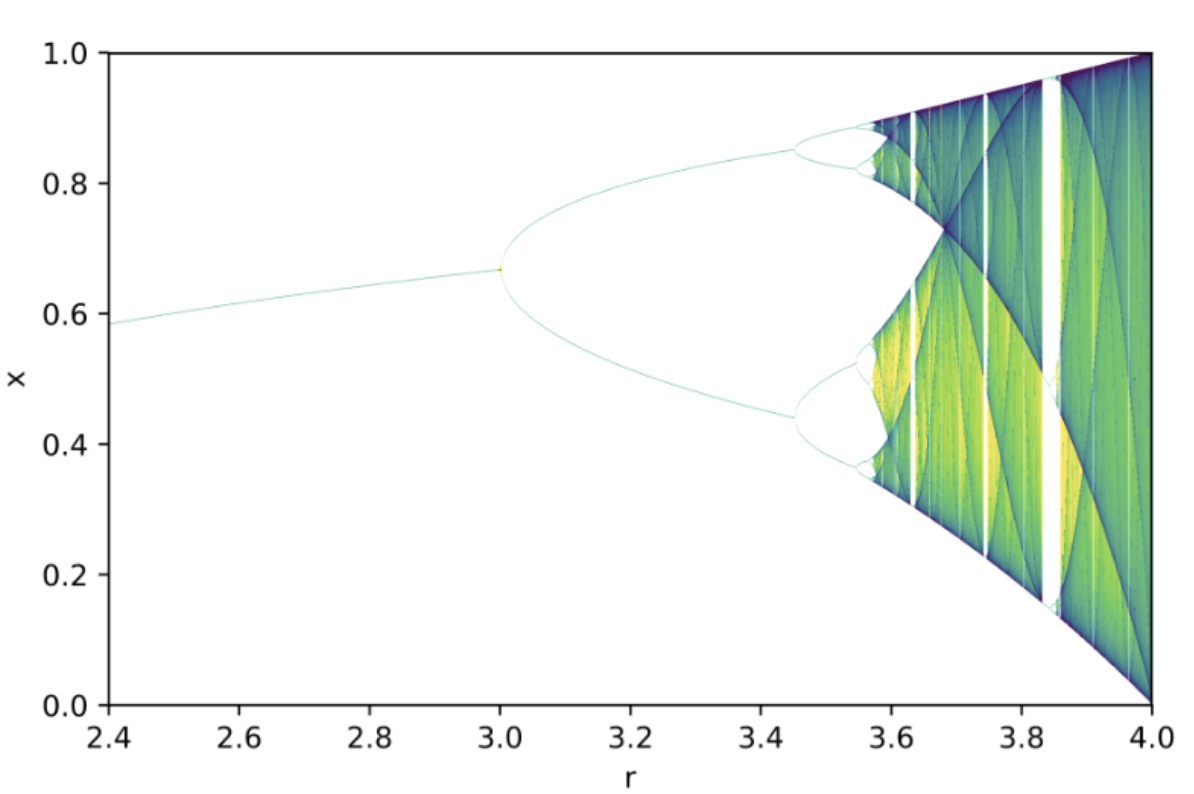
\includegraphics[width=8cm]{bifurcation.png}
    \caption{Bifurcation Diagram}
    \label{fig:Bifurcation Diagram}
\end{figure}

Besides the main topics of discrete systems, we will also go on to talk about the approach we took to solve problems related to each topic. Within these results, it will be shown how each exercise also related to one another and all tied together in the end. 

\section{Approach}
While reading about discrete systems in chapter 40 of Bruce Shapiro's textbook \emph{Scientific Computation: Python 3 Hacking for Math Junkies}, we recognized how all the main topics in the chapter related to one another. Besides just knowing that the topics tied together, it is important to also be able to show how each topic in the chapter comes together by doing the concepts through the textbook exercises on our own.

\subsection{Tent Map}
The first concept portrayed was developing a tent map to help determine the locations of the fixed points in the given function. Tent maps are typically defined on a given interval and then a piece wise function is provided to show how many fixed points the tent map should have. An example of a tent map is shown in Figure 4:
\begin{figure}[htp]
    \centering
    \includegraphics[width=8cm]{Carli Provide Tent Map from Exercise 6}
    \caption{This shows what a tent map should look like}
    \label{fig:Tent Map}
\end{figure}

\subsection{Bifurcation Diagram}
After providing the locations of the fixed points of a tent map, we were asked to provide a bifurcation diagram of the logistic map. A logistic map is similar to a tent map, in which it helps show where fixed points should occur. idk what else to write here so please continue:)

\end{document}
